\section{Nathaniel Laurente}

\subsection{Goal Statement}
    I worked on coming up with a Goal Statement that fits the new project.

\subsection{ESP32-C3 Communication With OLED Display}


\begin{figure}[!ht]
    \centering
    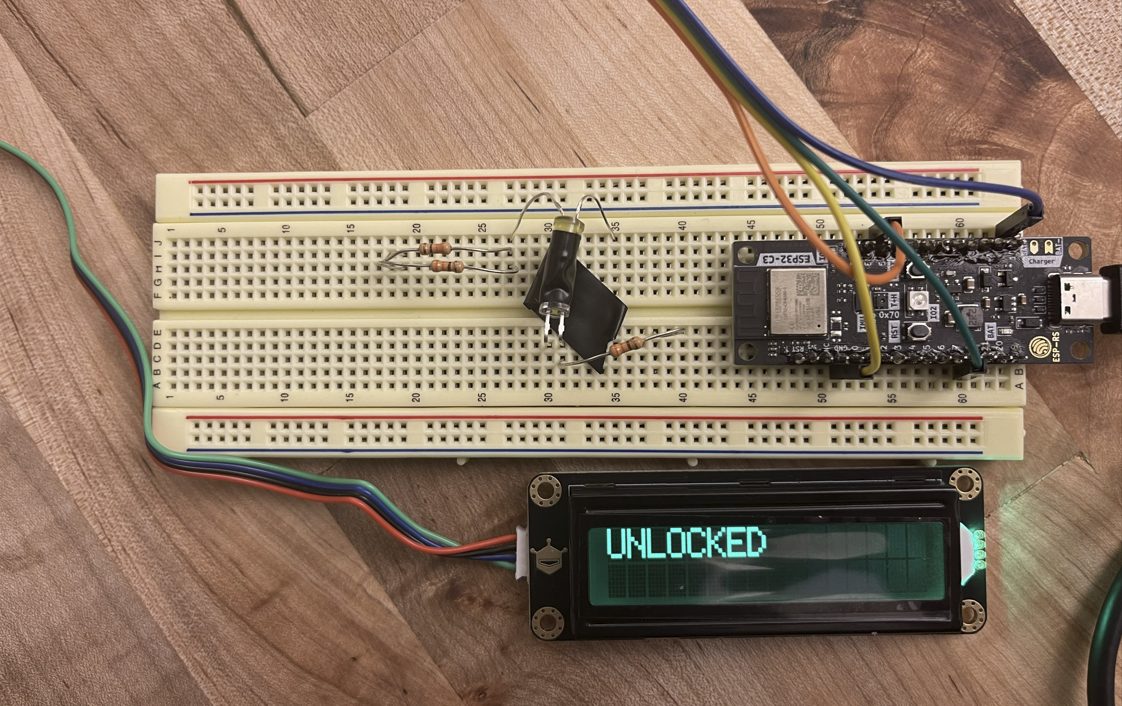
\includegraphics[width=140mm,scale=0.5]{./img/disp.png}
    \caption{ESP32-C3 Established Communication with OLED RGB Display}
    \label{fig:enter-label}
\end{figure}

    I was able to configure the ESP32-C3 to display "Unlocked" and "Locked." I set the toolchains such that there will be no issue sending signals from ESP32-C3 too the OLED dislay with minimal delay. My testing interface involved making sure there were no leaks and data was being power efficient when sending signals.

\subsection{Design For Manufacture}
    In the design for manufacture, I meticulously evaluated and selected components that strike an optimal balance between power efficiency and cost-effectiveness. This careful selection ensures that our auto-locking door system is not only marketable but also operates with minimal power consumption, thereby enhancing its overall functionality and sustainability.

\subsection{Decision Tables}
    I made the decision tables for the weights of the necessary parameters for our auto-locking door. This allowed our team to decide on a final design out of the three options we had come up with for our design. For an auto-locking door design, of course security was the number 1 concern for our project, and we decided to go for an option that prioritized security while maintaining cost efficiency.
